\chapter{Teoretický základ}
\label{2-teorie}

Tato kapitola si klade za cíl seznámit čtenáře s~teoretickými základy měření radioaktivity, z~nichž
plyne potřeba posunu. Dále pak načrtne způsoby, kterými bude možno body posouvat, a~popíše
nejdůležitější problémy, s nimiž se při takovém posunu lze setkat. 

\section{Scintilační spektrometrie}
\label{spektrometrie}

\subsection{Detektorová část}
\label{detektor}

\subsubsection{Scintilační krystal}
\label{krystal}

\subsubsection{Fotonásobič}
\label{fotonasobic}

\subsection{Analyzační část}
\label{analyzator}


\section{Sběr souřadnic a potřeba posunu}
\label{potreba posunu}


\section{Posun}
\label{posun}


\section{Problémy}
\label{problemy}

\subsection{Elipsoid}
\label{elipsoid}




\subsection{První geodetická úloha}
\label{prvnigu}

První geodetická úloha představuje hledání (výpočet) parametrů bodu na konci křivky, v~případě
představovaného zásuvného modulu na referenčním elipsoid. Zná\-mými parametry jsou souřadnice počátečního
bodu křivky a~její azimut v~tomto bodě. Hledanými parametry zeměpisné souřadnice koncového bodu.
Zkoumaná křivka reprezentuje geodetickou křivku. 

Základní geodetické úlohy se dají řešit nejedním způsobem a~v~minulosti vždy znamenaly mnohé potíže
a~dlouhé výpočty. S~rozvojem informačních technologií došlo k~značnému urychlení výpočtu.
Prezentovaný princip vychází z~principu popisovaného v~\cite{vyssigeodezie} a~vycházejícího
z~postupu Ing.~Jana Douši. 

Postup spočívá v~rozdělení křivky na integrační kroky. Křivku, resp.~její úsek~\textit{h}
aproximujeme polynomem čtvrtého stupně, takzvanou Runge-Kuttovou metodou řádu~4. Potíž spočívá v~tom,
na kolik úseků máme danou křivku rozdělit. Přesnost totiž ovlivňuje nejen délka křivky, ale také její
poloha na elipsoidu. 

Daný problém řeší postupné iterace. Křivka se postupně půlí, následně se půlí její poloviny atd. (jde
tedy o~\textit{1/n}~násobky původní délky, kde \textit{n} představuje mocniny dvou), než dosáhneme
požadované přesnosti. Ta je kontrolována pomocí podmínky cyklu: Pokud se od sebe všechny vypočtené
atributy koncového bodu křivky ve dvou po sobě jdoucích iteracích liší o~hodnotu menší než danou
(v našem případě 0.0000000001~úhlového stupně), jsou poslední vypočtené atributy brány jako výsledné. 


  \begin{figure}[H]
   \centering
	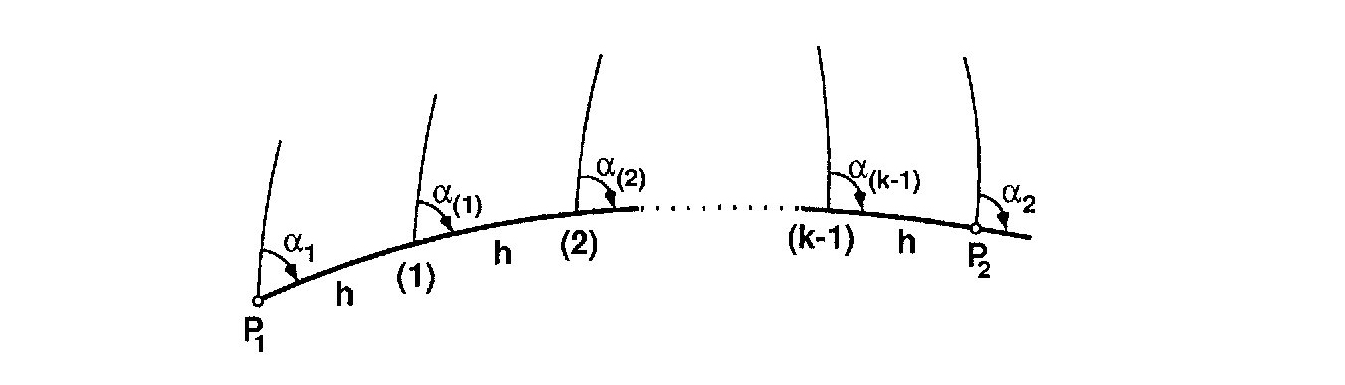
\includegraphics[scale=0.5]{./pictures/prvnigu-integrace.png}
	\caption[Integrační kroky v první geodetické úloze]{Integrační kroky v první geodetické úloze
	(zdroj: \cite{vyssigeodezie})}
      \label{fig:prvnigu-integrace}
  \end{figure}





